\chapter{Mastering the grammar}\label{cha:mastery}

\section{Introduction}\label{introduction}

In order to unlock the full power of ggplot2, you'll need to master the
underlying grammar. By understanding the grammar, and how its components
fit together, you can create a wider range of visualizations, combine
multiple sources of data, and customise to your heart's content.

This chapter describes the theoretical basis of ggplot2: the layered
grammar of graphics. The layered grammar is based on Wilkinson's grammar
of graphics (Wilkinson 2005), but adds a number of enhancements that
help it to be more expressive and fit seamlessly into the R environment.
The differences between the layered grammar and Wilkinson's grammar are
described fully in Wickham (2008). In this chapter you will learn a
little bit about each component of the grammar and how they all fit
together. The next chapters discuss the components in more detail, and
provide more examples of how you can use them in practice.
\index{Grammar!theory}

The grammar makes it easier for you to iteratively update a plot,
changing a single feature at a time. The grammar is also useful because
it suggests the high-level aspects of a plot that \emph{can} be changed,
giving you a framework to think about graphics, and hopefully shortening
the distance from mind to paper. It also encourages the use of graphics
customised to a particular problem, rather than relying on specific
chart types.

This chapter begins by describing in detail the process of drawing a
simple plot. \protect\hyperlink{sec:simple-plot}{Building a scatterplot}
starts with a simple scatterplot, then
\protect\hyperlink{sec:complex-plot}{Adding complexity} makes it more
complex by adding a smooth line and facetting. While working through
these examples you will be introduced to all six components of the
grammar, which are then defined more precisely in
\protect\hyperlink{sec:components}{Components of the layered grammar}.

\hypertarget{sec:simple-plot}{\section{Building a
scatterplot}\label{sec:simple-plot}}

How are engine size and fuel economy related? We might create a
scatterplot of engine displacement and highway mpg with points coloured
by number of cylinders:

\begin{Shaded}
\begin{Highlighting}[]
\KeywordTok{ggplot}\NormalTok{(mpg, }\KeywordTok{aes}\NormalTok{(displ, hwy, }\DataTypeTok{colour =} \KeywordTok{factor}\NormalTok{(cyl))) +}
\StringTok{  }\KeywordTok{geom_point}\NormalTok{()}
\end{Highlighting}
\end{Shaded}

\begin{figure}[H]
  \centering
  \includegraphics[width=0.65\linewidth]{_figures/mastery/unnamed-chunk-1-1}
\end{figure}

You can create plots like this easily, but what is going on underneath
the surface? How does ggplot2 draw this plot?
\index{Scatterplot!principles of}

\subsection{Mapping aesthetics to
data}\label{mapping-aesthetics-to-data}

What precisely is a scatterplot? You have seen many before and have
probably even drawn some by hand. A scatterplot represents each
observation as a point, positioned according to the value of two
variables. As well as a horizontal and vertical position, each point
also has a size, a colour and a shape. These attributes are called
\textbf{aesthetics}, and are the properties that can be perceived on the
graphic. Each aesthetic can be mapped to a variable, or set to a
constant value. In the previous graphic, \texttt{displ} is mapped to
horizontal position, \texttt{hwy} to vertical position and \texttt{cyl}
to colour. Size and shape are not mapped to variables, but remain at
their (constant) default values. \index{Aesthetics!mapping}

Once we have these mappings we can create a new dataset that records
this information:

\begin{longtable}[c]{@{}rrr@{}}
\toprule
x & y & colour\tabularnewline
\midrule
\endhead
1.8 & 29 & 4\tabularnewline
1.8 & 29 & 4\tabularnewline
2.0 & 31 & 4\tabularnewline
2.0 & 30 & 4\tabularnewline
2.8 & 26 & 6\tabularnewline
2.8 & 26 & 6\tabularnewline
3.1 & 27 & 6\tabularnewline
1.8 & 26 & 4\tabularnewline
\bottomrule
\end{longtable}

This new dataset is a result of applying the aesthetic mappings to the
original data. We can create many different types of plots using this
data. The scatterplot uses points, but were we instead to draw lines we
would get a line plot. If we used bars, we'd get a bar plot. Neither of
those examples makes sense for this data, but we could still draw them
(I've omitted the legends to save space):

\begin{Shaded}
\begin{Highlighting}[]
\KeywordTok{ggplot}\NormalTok{(mpg, }\KeywordTok{aes}\NormalTok{(displ, hwy, }\DataTypeTok{colour =} \KeywordTok{factor}\NormalTok{(cyl))) +}
\StringTok{  }\KeywordTok{geom_line}\NormalTok{() +}\StringTok{ }
\StringTok{  }\KeywordTok{theme}\NormalTok{(}\DataTypeTok{legend.position =} \StringTok{"none"}\NormalTok{)}
\KeywordTok{ggplot}\NormalTok{(mpg, }\KeywordTok{aes}\NormalTok{(displ, hwy, }\DataTypeTok{colour =} \KeywordTok{factor}\NormalTok{(cyl))) +}
\StringTok{  }\KeywordTok{geom_bar}\NormalTok{(}\DataTypeTok{stat =} \StringTok{"identity"}\NormalTok{, }\DataTypeTok{position =} \StringTok{"identity"}\NormalTok{, }\DataTypeTok{fill =} \OtherTok{NA}\NormalTok{) +}\StringTok{ }
\StringTok{  }\KeywordTok{theme}\NormalTok{(}\DataTypeTok{legend.position =} \StringTok{"none"}\NormalTok{)}
\end{Highlighting}
\end{Shaded}

\begin{figure}[H]
  \includegraphics[width=0.5\linewidth]{_figures/mastery/other-geoms-1}%
  \includegraphics[width=0.5\linewidth]{_figures/mastery/other-geoms-2}
\end{figure}

In ggplot, we can produce many plots that don't make sense, yet are
grammatically valid. This is no different than English, where we can
create senseless but grammatical sentences like the angry rock barked
like a comma.

Points, lines and bars are all examples of geometric objects, or
\textbf{geoms}. Geoms determine the ``type'' of the plot. Plots that use
a single geom are often given a special name:

\begin{longtable}[c]{@{}lll@{}}
\toprule
Named plot & Geom & Other features\tabularnewline
\midrule
\endhead
scatterplot & point &\tabularnewline
bubblechart & point & size mapped to a variable\tabularnewline
barchart & bar &\tabularnewline
box-and-whisker plot & boxplot &\tabularnewline
line chart & line &\tabularnewline
\bottomrule
\end{longtable}

More complex plots with combinations of multiple geoms don't have a
special name, and we have to describe them by hand. For example, this
plot overlays a per group regression line on top of a scatterplot:

\begin{Shaded}
\begin{Highlighting}[]
\KeywordTok{ggplot}\NormalTok{(mpg, }\KeywordTok{aes}\NormalTok{(displ, hwy, }\DataTypeTok{colour =} \KeywordTok{factor}\NormalTok{(cyl))) +}\StringTok{ }
\StringTok{  }\KeywordTok{geom_point}\NormalTok{() +}\StringTok{ }
\StringTok{  }\KeywordTok{geom_smooth}\NormalTok{(}\DataTypeTok{method =} \StringTok{"lm"}\NormalTok{)}
\end{Highlighting}
\end{Shaded}

\begin{figure}[H]
  \centering
  \includegraphics[width=0.65\linewidth]{_figures/mastery/complex-plot-1}
\end{figure}

What would you call this plot? Once you've mastered the grammar, you'll
find that many of the plots that you produce are uniquely tailored to
your problems and will no longer have special names. \index{Named plots}

\subsection{Scaling}\label{scaling}

The values in the previous table have no meaning to the computer. We
need to convert them from data units (e.g., litres, miles per gallon and
number of cylinders) to graphical units (e.g., pixels and colours) that
the computer can display. This conversion process is called
\textbf{scaling} and performed by scales. Now that these values are
meaningful to the computer, they may not be meaningful to us: colours
are represented by a six-letter hexadecimal string, sizes by a number
and shapes by an integer. These aesthetic specifications that are
meaningful to R are described in \texttt{vignette("ggplot2-specs")}.
\index{Scales!introduction}

In this example, we have three aesthetics that need to be scaled:
horizontal position (\texttt{x}), vertical position (\texttt{y}) and
\texttt{colour}. Scaling position is easy in this example because we are
using the default linear scales. We need only a linear mapping from the
range of the data to \([0, 1]\). We use \([0, 1]\) instead of exact
pixels because the drawing system that ggplot2 uses, \textbf{grid},
takes care of that final conversion for us. A final step determines how
the two positions (x and y) are combined to form the final location on
the plot. This is done by the coordinate system, or \textbf{coord}. In
most cases this will be Cartesian coordinates, but it might be polar
coordinates, or a spherical projection used for a map.

The process for mapping the colour is a little more complicated, as we
have a non-numeric result: colours. However, colours can be thought of
as having three components, corresponding to the three types of
colour-detecting cells in the human eye. These three cell types give
rise to a three-dimensional colour space. Scaling then involves mapping
the data values to points in this space. There are many ways to do this,
but here since \texttt{cyl} is a categorical variable we map values to
evenly spaced hues on the colour wheel, as shown in Figure
\ref{fig:colour-wheel}. A different mapping is used when the variable is
continuous. \index{Colour!wheel}

\begin{figure}[htbp]
  \centering
    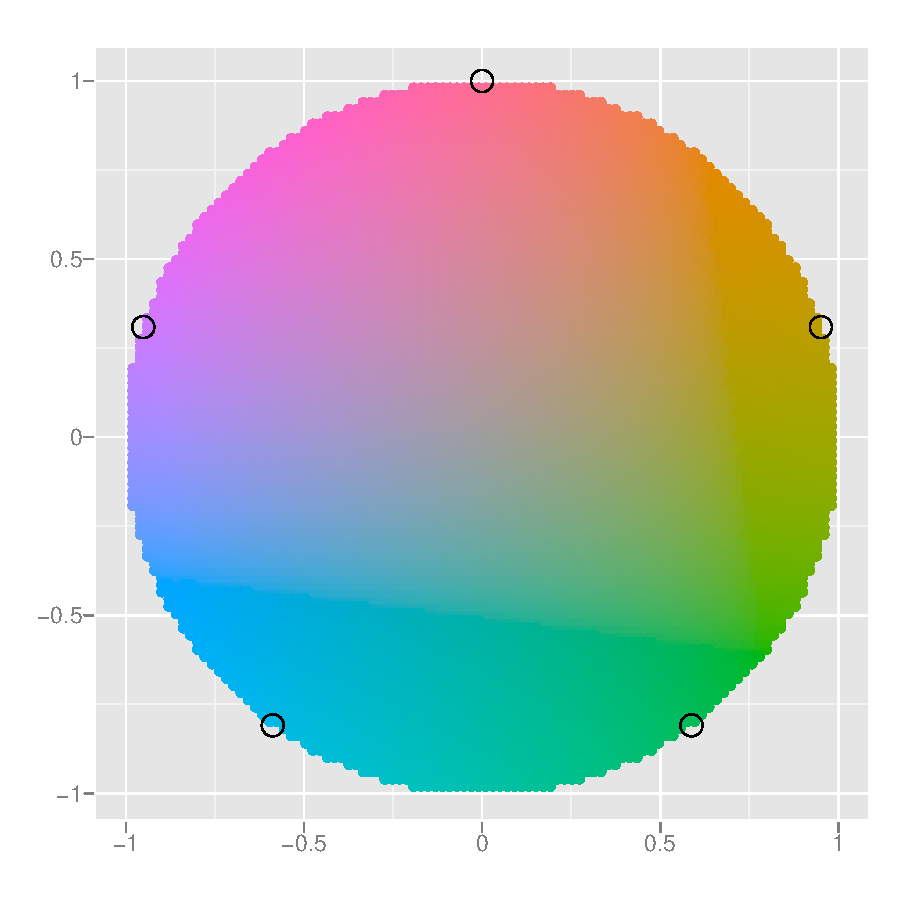
\includegraphics[width=2in]{diagrams/colour-wheel}
  \caption{A colour wheel illustrating the choice of five equally spaced colours. This is the default scale for discrete variables.}
  \label{fig:colour-wheel}
\end{figure}

The result of these conversions is below. As well as aesthetics that
have been mapped to variable, we also include aesthetics that are
constant. We need these so that the aesthetics for each point are
completely specified and R can draw the plot. The points will be filled
circles (shape 19 in R) with a 1-mm diameter:

\begin{longtable}[c]{@{}lllll@{}}
\toprule
x & y & colour & size & shape\tabularnewline
\midrule
\endhead
0.037 & 0.531 & \#F8766D & 1 & 19\tabularnewline
0.037 & 0.531 & \#F8766D & 1 & 19\tabularnewline
0.074 & 0.594 & \#F8766D & 1 & 19\tabularnewline
0.074 & 0.562 & \#F8766D & 1 & 19\tabularnewline
0.222 & 0.438 & \#00BFC4 & 1 & 19\tabularnewline
0.222 & 0.438 & \#00BFC4 & 1 & 19\tabularnewline
0.278 & 0.469 & \#00BFC4 & 1 & 19\tabularnewline
0.037 & 0.438 & \#F8766D & 1 & 19\tabularnewline
\bottomrule
\end{longtable}

Finally, we need to render this data to create the graphical objects
that are displayed on the screen. To create a complete plot we need to
combine graphical objects from three sources: the \emph{data},
represented by the point geom; the \emph{scales and coordinate system},
which generate axes and legends so that we can read values from the
graph; and \emph{plot annotations}, such as the background and plot
title.

\hypertarget{sec:complex-plot}{\section{Adding
complexity}\label{sec:complex-plot}}

With a simple example under our belts, let's now turn to look at this
slightly more complicated example:

\begin{Shaded}
\begin{Highlighting}[]
\KeywordTok{ggplot}\NormalTok{(mpg, }\KeywordTok{aes}\NormalTok{(displ, hwy)) +}\StringTok{ }
\StringTok{  }\KeywordTok{geom_point}\NormalTok{() +}
\StringTok{  }\KeywordTok{geom_smooth}\NormalTok{() +}\StringTok{ }
\StringTok{  }\KeywordTok{facet_wrap}\NormalTok{(~year)}
\end{Highlighting}
\end{Shaded}

\begin{figure}[H]
  \centering
  \includegraphics[width=0.75\linewidth]{_figures/mastery/complex-1}
\end{figure}

This plot adds three new components to the mix: facets, multiple layers
and statistics. The facets and layers expand the data structure
described above: each facet panel in each layer has its own dataset. You
can think of this as a 3d array: the panels of the facets form a 2d
grid, and the layers extend upwards in the 3rd dimension. In this case
the data in the layers is the same, but in general we can plot different
datasets on different layers.

The smooth layer is different to the point layer because it doesn't
display the raw data, but instead displays a statistical transformation
of the data. Specifically, the smooth layer fits a smooth line through
the middle of the data. This requires an additional step in the process
described above: after mapping the data to aesthetics, the data is
passed to a statistical transformation, or \textbf{stat}, which
manipulates the data in some useful way. In this example, the stat fits
the data to a loess smoother, and then returns predictions from evenly
spaced points within the range of the data. Other useful stats include 1
and 2d binning, group means, quantile regression and contouring.

As well as adding an additional step to summarise the data, we also need
some extra steps when we get to the scales. This is because we now have
multiple datasets (for the different facets and layers) and we need to
make sure that the scales are the same across all of them. Scaling
actually occurs in three parts: transforming, training and mapping. We
haven't mentioned transformation before, but you have probably seen it
before in log-log plots. In a log-log plot, the data values are not
linearly mapped to position on the plot, but are first log-transformed.

\begin{itemize}
\item
  Scale transformation occurs before statistical transformation so that
  statistics are computed on the scale-transformed data. This ensures
  that a plot of \(\log(x)\) vs. \(\log(y)\) on linear scales looks the
  same as \(x\) vs. \(y\) on log scales. There are many different
  transformations that can be used, including taking square roots,
  logarithms and reciprocals. See
  \protect\hyperlink{sub:scale-position}{continuous scales} for more
  details.
\item
  After the statistics are computed, each scale is trained on every
  dataset from all the layers and facets. The training operation
  combines the ranges of the individual datasets to get the range of the
  complete data. Without this step, scales could only make sense locally
  and we wouldn't be able to overlay different layers because their
  positions wouldn't line up. Sometimes we do want to vary position
  scales across facets (but never across layers), and this is described
  more fully in \protect\hyperlink{sub:controlling-scales}{controlling
  scales}.
\item
  Finally the scales map the data values into aesthetic values. This is
  a local operation: the variables in each dataset are mapped to their
  aesthetic values, producing a new dataset that can then be rendered by
  the geoms.
\end{itemize}

Figure \ref{fig:schematic} illustrates the complete process
schematically.

\begin{figure}[htbp]
  \centering
  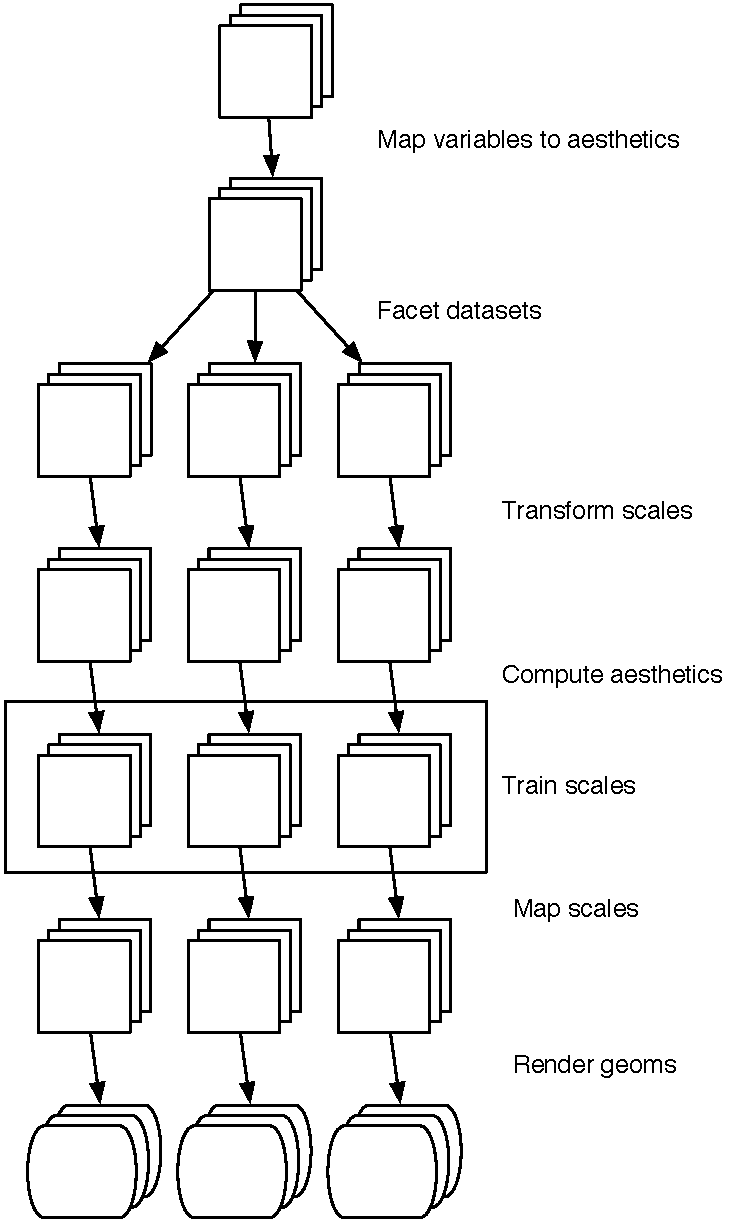
\includegraphics[width=4in]{diagrams/mastery-schema}
  \caption{Schematic description of the plot generation process. Each square represents a layer, and this schematic represents a plot with three layers and three panels. All steps work by transforming individual data frames except for training scales, which doesn't affect the data frame and operates across all datasets simultaneously.}
  \label{fig:schematic}
\end{figure}

\hypertarget{sec:components}{\section{Components of the layered
grammar}\label{sec:components}}

In the examples above, we have seen some of the components that make up
a plot: data and aesthetic mappings, geometric objects (geoms),
statistical transformations (stats), scales, and facetting. We have also
touched on the coordinate system. One thing we didn't mention is the
position adjustment, which deals with overlapping graphic objects.
Together, the data, mappings, stat, geom and position adjustment form a
\textbf{layer}. A plot may have multiple layers, as in the example where
we overlaid a smoothed line on a scatterplot. All together, the layered
grammar defines a plot as the combination of: \index{Grammar!components}

\begin{itemize}
\item
  A default dataset and set of mappings from variables to aesthetics.
\item
  One or more layers, each composed of a geometric object, a statistical
  transformation, a position adjustment, and optionally, a dataset and
  aesthetic mappings.
\item
  One scale for each aesthetic mapping.
\item
  A coordinate system.
\item
  The facetting specification.
\end{itemize}

The following sections describe each of the higher-level components more
precisely, and point you to the parts of the book where they are
documented.

\subsection{Layers}\label{layers}

\textbf{Layers} are responsible for creating the objects that we
perceive on the plot. A layer is composed of five parts:

\begin{enumerate}
\def\labelenumi{\arabic{enumi}.}
\tightlist
\item
  Data
\item
  Aesthetic mappings.
\item
  A statistical transformation (stat).
\item
  A geometric object (geom).
\item
  A position adjustment.
\end{enumerate}

The properties of a layer are described in
\protect\hyperlink{cha:layers}{layers} and their uses for data
visualisation in \protect\hyperlink{cha:toolbox}{toolbox}.

\subsection{Scales}\label{sub:scales}

A \textbf{scale} controls the mapping from data to aesthetic attributes,
and we need a scale for every aesthetic used on a plot. Each scale
operates across all the data in the plot, ensuring a consistent mapping
from data to aesthetics. Some examples are shown in Figure
\ref{fig:scale-legends}.

\begin{figure}[H]
  \includegraphics[width=1\linewidth]{_figures/mastery/scale-legends-1}
  \caption{Examples of legends from four different scales. From left to right: continuous variable mapped to size, and to colour, discrete variable mapped to shape, and to colour. The ordering of scales seems upside-down, but this matches the labelling of the $y$-axis: small values occur at the bottom.}
  \label{fig:scale-legends}
\end{figure}

A scale is a function and its inverse, along with a set of parameters.
For example, the colour gradient scale maps a segment of the real line
to a path through a colour space. The parameters of the function define
whether the path is linear or curved, which colour space to use (e.g.,
LUV or RGB), and the colours at the start and end.

The inverse function is used to draw a guide so that you can read values
from the graph. Guides are either axes (for position scales) or legends
(for everything else). Most mappings have a unique inverse (i.e., the
mapping function is one-to-one), but many do not. A unique inverse makes
it possible to recover the original data, but this is not always
desirable if we want to focus attention on a single aspect.

For more details, see \protect\hyperlink{cha:scales}{scales chapter}.

\subsection{Coordinate system}\label{sub:coordinate-systems}

A coordinate system, or \textbf{coord} for short, maps the position of
objects onto the plane of the plot. Position is often specified by two
coordinates \((x, y)\), but potentially could be three or more (although
this is not implemented in ggplot2). The Cartesian coordinate system is
the most common coordinate system for two dimensions, while polar
coordinates and various map projections are used less frequently.

Coordinate systems affect all position variables simultaneously and
differ from scales in that they also change the appearance of the
geometric objects. For example, in polar coordinates, bar geoms look
like segments of a circle. Additionally, scaling is performed before
statistical transformation, while coordinate transformations occur
afterward. The consequences of this are shown in
\protect\hyperlink{sub:coord-non-linear}{coordinate transformations}.

Coordinate systems control how the axes and grid lines are drawn. Figure
\ref{fig:coord} illustrates three different types of coordinate systems.
Very little advice is available for drawing these for non-Cartesian
coordinate systems, so a lot of work needs to be done to produce
polished output. See \protect\hyperlink{sec:coord}{coordinate systems}
for more details.

\begin{figure}[H]
  \includegraphics[width=0.333\linewidth]{_figures/mastery/coord-1}%
  \includegraphics[width=0.333\linewidth]{_figures/mastery/coord-2}%
  \includegraphics[width=0.333\linewidth]{_figures/mastery/coord-3}
  \caption{Examples of axes and grid lines for three coordinate systems: Cartesian, semi-log and polar. The polar coordinate system illustrates the difficulties associated with non-Cartesian coordinates: it is hard to draw the axes well.}
  \label{fig:coord}
\end{figure}

\subsection{Facetting}\label{sub:intro-facetting}

There is also another thing that turns out to be sufficiently useful
that we should include it in our general framework: facetting, a general
case of conditioned or trellised plots. This makes it easy to create
small multiples, each showing a different subset of the whole dataset.
This is a powerful tool when investigating whether patterns hold across
all conditions. The facetting specification describes which variables
should be used to split up the data, and whether position scales should
be free or constrained. Facetting is described in
\protect\hyperlink{cha:position}{position}.

\section{Exercises}\label{exercises}

\begin{enumerate}
\def\labelenumi{\arabic{enumi}.}
\item
  One of the best ways to get a handle on how the grammar works is to
  apply it to the analysis of existing graphics. For each of the
  graphics listed below, write down the components of the graphic. Don't
  worry if you don't know what the corresponding functions in ggplot2
  are called (or if they even exist!), instead focussing on recording
  the key elements of a plot so you could communicate it to someone
  else.

  \begin{enumerate}
  \def\labelenumii{\arabic{enumii}.}
  \item
    ``Napoleon's march'' by Charles John Minard:
    \url{http://www.datavis.ca/gallery/re-minard.php}
  \item
    ``Where the Heat and the Thunder Hit Their Shots'', by Jeremy White,
    Joe Ward, and Matthew Ericson at The New York Times.
    \url{http://nyti.ms/1duzTvY}
  \item
    ``London Cycle Hire Journeys'', by James Cheshire.
    \url{http://bit.ly/1S2cyRy}
  \item
    The Pew Research Center's favorite data visualizations of 2014:
    \url{http://pewrsr.ch/1KZSSN6}
  \item
    ``The Tony's Have Never Been so Dominated by Women'', by Joanna Kao
    at FiveThirtyEight: \url{http://53eig.ht/1cJRCyG}.
  \item
    ``In Climbing Income Ladder, Location Matters'' by the Mike Bostock,
    Shan Carter, Amanda Cox, Matthew Ericson, Josh Keller, Alicia
    Parlapiano, Kevin Quealy and Josh Williams at the New York Times:
    \url{http://nyti.ms/1S2dJQT}
  \item
    ``Dissecting a Trailer: The Parts of the Film That Make the Cut'',
    by Shan Carter, Amanda Cox, and Mike Bostock at the New York Times:
    \url{http://nyti.ms/1KTJQOE}
  \end{enumerate}
\end{enumerate}

\section*{References}\label{references}
\addcontentsline{toc}{section}{References}

\hypertarget{refs}{}
\hypertarget{ref-wickham:2008}{}
Wickham, Hadley. 2008. ``Practical Tools for Exploring Data and
Models.'' PhD thesis, Iowa State University.
\url{http://had.co.nz/thesis}.

\hypertarget{ref-wilkinson:2006}{}
Wilkinson, Leland. 2005. \emph{The Grammar of Graphics}. 2nd ed.
Statistics and Computing. Springer.
